The well known \textit{Brezzi-BabÃŒska} condition (also called \textit{inf-sup} condition) determinates the interpolation families for the velocity and pressure to ensure stability and convergence in the Stokes problem. Originally, the PFEM-2 method uses the family P1/P1 (linear triangular elements) to approximate the variables $\mathbf{u}$ and $p$ on the mesh\cite{Idelsohn12b}. % because is a computationally cheap approach.
However, this family does not satisfy the \textit{inf-sup} condition, then it is unstable, so it requires to use stabilization at the Poisson step. Maybe carrying on the extra cost of the stabilization is possible, but using linear elements does not provided good accuracy with coarser meshes. Using finer meshes in PFEM-2 introduce another extra cost due to the necessity for use more particles to approximate the fields and update nodal values.

An alternative proposal is presented in this report. The idea is using the called Taylor-Hood finite elements\cite{HoodTaylor73}, which are presented in Figure \ref{fg:taylor-hood}. They consist on a quadratic approximation for the velocity and continuous linear approximation for pressure (family P2/P1). It is demonstrated that this family is stable because it satisfies the \textit{inf-sup} condition. However, that advantage could not be useful if the cpu-time required to reach some accuracy is larger than using P1/P1 elements.

\begin{figure}[htbp]
  \begin{center}
      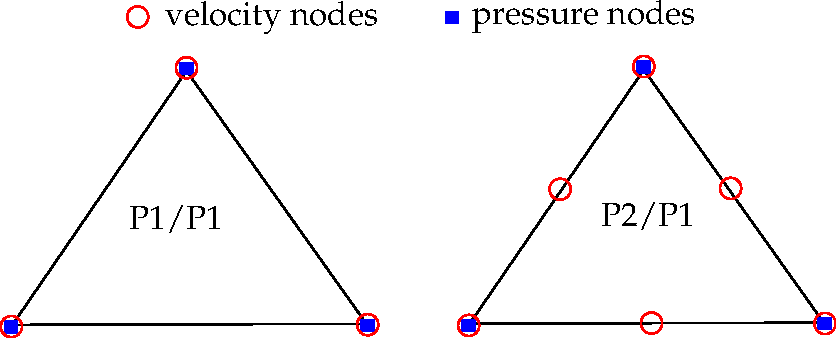
\includegraphics[width=.9\columnwidth]{images/taylor_hood.pdf}
  \end{center}
  \caption{\label{fg:taylor-hood} Left: Family P1/P1 originally used by PFEM-2. Right: Family P2/P1 proposed by this work.}
\end{figure}

\subsection{Square Cavity Tests}
% Previously, a new strategy to assemble the matrices and vectors of the linear equation systems was developed. It consists of pre-assembling the global matrices at the beginning of the simulation (for example mass and stiffness matrices), and after, at each time-step performing the final assemble with matrix-vector products. This approach improves the efficiency of the previous code (which assemble the matrices doing a loop over all the elements each time-step) in about a 20\%. However, it remains testing problems with variable coefficients.

% As we will see later, this approach is not useful for multi-fluids simulations, because the elemental matrices must be assembled each time-step and that formulation depends on the fluid zone that the element represents (interface zone or not).

Cartesian meshes were used for all cases. The name of the meshes indicates how many vertex-nodes there are in x-direction and y-direction respectly. For example the mesh \texttt{50x50-1ºorder} has 50 vertex-nodes in x-axis and 50 vertex-nodes in y-axis, conforming around 4800 first order triangular elements with 2500 degrees of freedom per variable. With second order grids have similar criteria, for example \texttt{25x25-2ºorder} has 25 vertex-nodes in each direction conforming 1250 second order triangular elements with approximately 2601 degrees of freedom per variable. Therefore the equation systems to solve with those meshes have approximately the same size.

\subsubsection{Re1000}

It was simulated using $\Delta t = 0.02$. Final simulation time $t_{final} = 50[s]$.

\begin{figure}[htbp]
  \begin{center}
      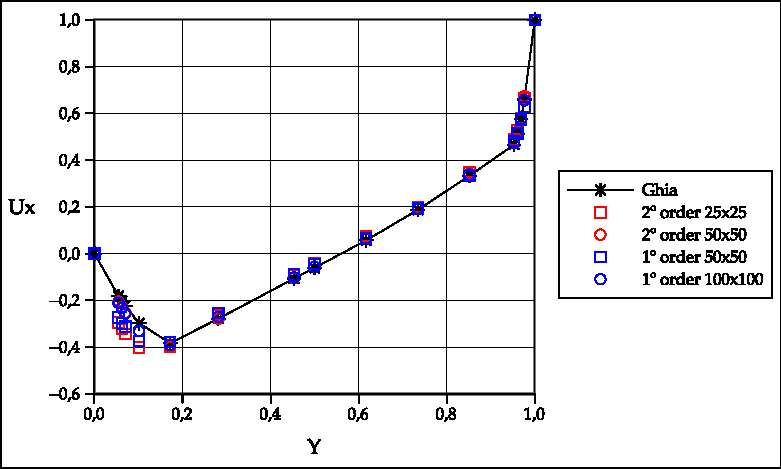
\includegraphics[width=.85\linewidth]{images/Re_1000_Ux.pdf}
      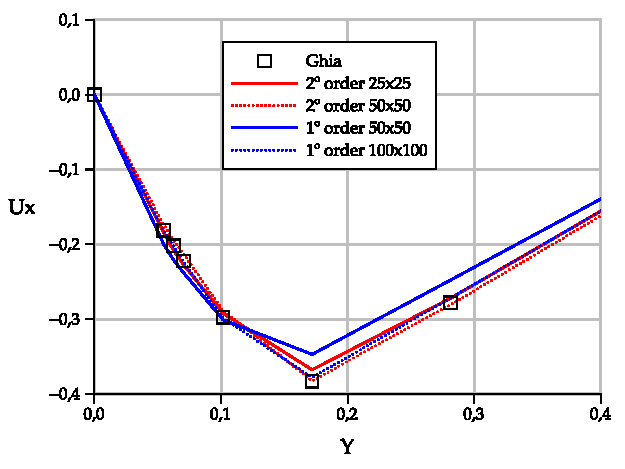
\includegraphics[width=.85\linewidth]{images/Re_1000_Ux_zoom.pdf}
  \end{center}
  \caption{\label{fg:Re1000u} Comparison with Ghia References at $Re=1000$. $u$ velocities at x-centerline.}
\end{figure}

\begin{figure}[htbp]
  \begin{center}
      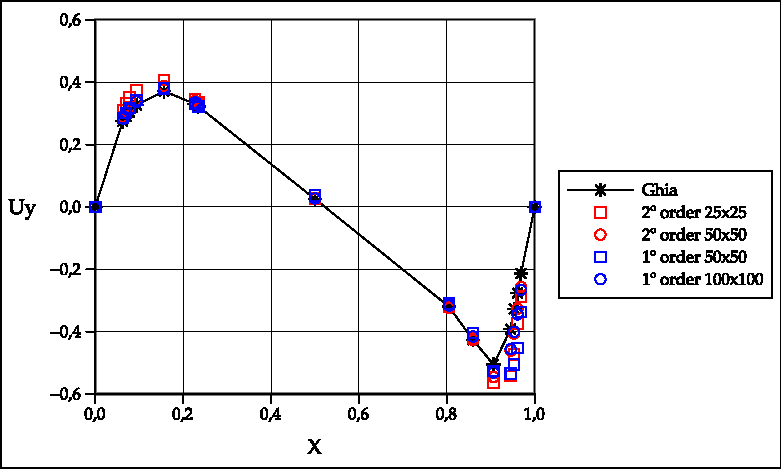
\includegraphics[width=.85\linewidth]{images/Re_1000_Uy.pdf}
      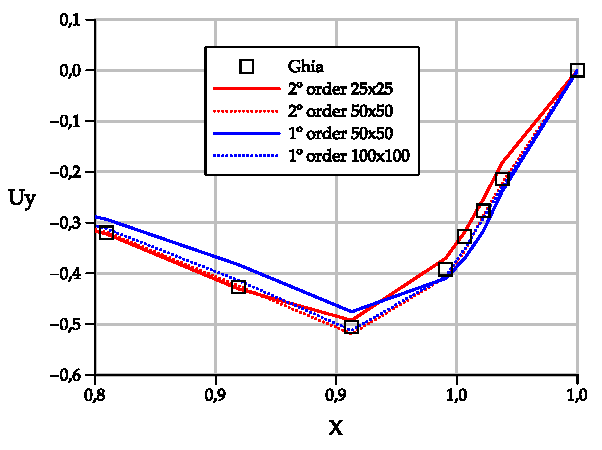
\includegraphics[width=.85\linewidth]{images/Re_1000_Uy_zoom.pdf}
  \end{center}
  \caption{\label{fg:Re1000v} Comparison with Ghia References at $Re=1000$. $v$ velocities at y-centerline.}
\end{figure}

\begin{table}[htbp]
\begin{center}
{\footnotesize
\begin{tabular}[h]{||c|c|c|c|c||}
    \hline
      Stage & $25x25$ - 2º order & $50x50$  - 2º order & $50x50$ - 1º order & $100x100$ - 1º order\\
      \hline
      \hline
	Acceleration & 34.6[s]& 134.58[s]& 22.8[s] & 97.9\\
	X-IVAS & 102.3[s]& 423.7[s]& 108.93[s] & 488.9 \\
	Projection & 32.4[s]& 153.8[s]& 75.0[s] & 359.1\\
	Poisson & 48.3[s]& 190.4[s]& 66.4[s] & 278.7\\
	Correction & 39.9[s]& 190.0[s]& 39.7[s] & 233.6\\
      \hline
	TOTAL & 257.57[s]& 1092.6[s]& 312.9[s] & 1458.1\\
      \hline
      \hline
	RMS $u$ & $2.0\times10^{-3}$ & $1.4\times10^{-3}$ & $5.8\times10^{-3}$ & $1.7\times10^{-3}$ \\
	RMS $v$ & $3.0\times10^{-3}$ & $2.2\times10^{-3}$ & $6.7\times10^{-3}$ & $2.4\times10^{-3}$ \\
      \hline
      \hline
\end{tabular}
}
\caption{\label{Tabla:times_Re_1000} Comparison table for CPU-times for the different PFEM-2 stages and the root mean square of the approximation error of $u$ and $v$. Case: $Re=1000$.}
\end{center}
\end{table}

\newpage

\subsubsection{Re 3200}


It was simulated using $\Delta t = 0.01$. Final simulation time $t_{final} = 100[s]$.

\begin{figure}[htbp]
  \begin{center}
      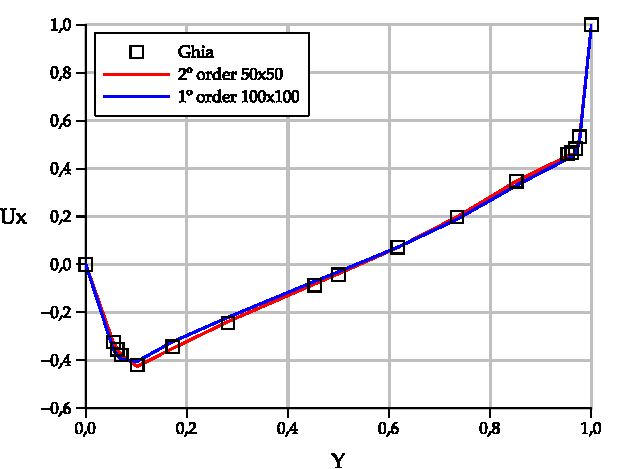
\includegraphics[width=.85\linewidth]{images/Re_3200_Ux.pdf}
      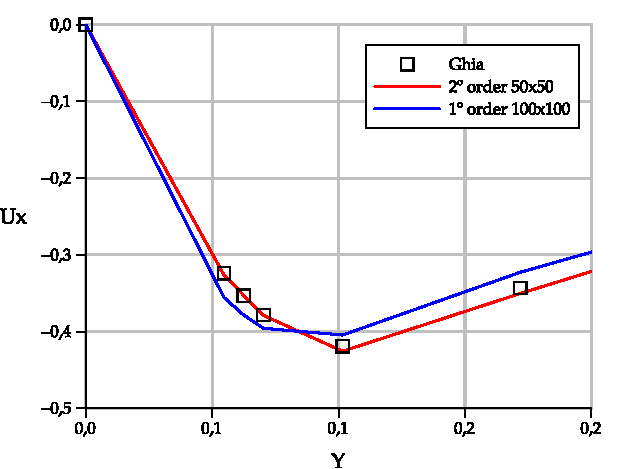
\includegraphics[width=.85\linewidth]{images/Re_3200_Ux_zoom.pdf}
  \end{center}
  \caption{\label{fg:Re3200} Comparison with Ghia References at $Re=3200$. $u$ velocities at x-centerline.}
\end{figure}

\begin{table}[htbp]
\begin{center}
{\footnotesize
\begin{tabular}[h]{||c|c|c||}
    \hline
      Stage & $50x50$  -2º order & $100x100$ - 1º order\\
      \hline
      \hline
	Acceleration & 134.9[s]& 98.01[s]\\
	X-IVAS & 427.5[s]& 499.9[s] \\
	Projection & 154.7[s]& 368.5\\
	Poisson & 191.1[s]& 283.6\\
	Correction & 189.2[s]& 242.9\\
      \hline
	TOTAL & 1097.4[s]& 1492.9\\
      \hline
      \hline
	RMS $u$ & 0.0106 & 0.0113 \\
      \hline
      \hline
\end{tabular}
}
\caption{\label{Tabla:times_Re_3200} Comparison table for CPU-times (to achieve $30[s]$ of real time) for the different PFEM-2 stages. Also the root mean square of the approximation error of $u$ at the end of the simulation is presented. Case: $Re=3200$.}
\end{center}
\end{table}

\newpage

\subsubsection{Re 10000}


It was simulated using $\Delta t = 0.01$. Final simulation time $t_{final} = 75[s]$.

\begin{figure}[htbp]
  \begin{center}
      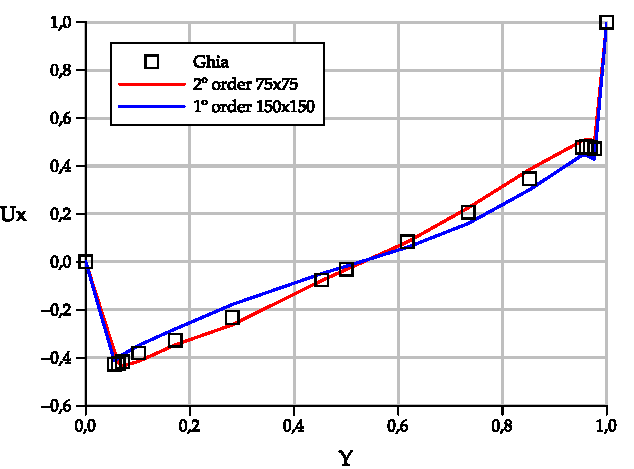
\includegraphics[width=.85\linewidth]{images/Re_10000_Ux.pdf}
  \end{center}
  \caption{\label{fg:Re10000} Comparison with Ghia References at $Re=10000$. $u$ velocities at x-centerline.}
\end{figure}


\begin{table}[htbp]
\begin{center}
{\footnotesize
\begin{tabular}[h]{||c|c|c||}
    \hline
      Stage & $75x75$  -2º order & $150x150$ - 1º order\\
      \hline
      \hline
	Acceleration & 515.0[s]& 367.1[s]\\
	X-IVAS & 1741.2[s]& 2114.1[s] \\
	Projection & 731.5[s]& 1651.2[s]\\
	Poisson & 740.9[s]& 1078.6[s]\\
	Correction & 911.4[s]& 1237.9[s]\\
      \hline
	TOTAL & 4640.0[s]& 6449.0[s]\\
      \hline
      \hline
	RMS $u$ & 0.015 & 0.0213 \\
      \hline
      \hline
\end{tabular}
}
\caption{\label{Tabla:times_Re_10000} Comparison table for CPU-times for the different PFEM-2 stages and the root mean square of the approximation error of $u$. Case: $Re=10000$.}
\end{center}
\end{table}

\newpage

\subsection{Summary}

  \begin{itemize}
   \item With the same number of nodes, second order achieve better accuracy than first order.
   \item With the same number of nodes, second order might be more efficient (it requires less elements and, then, less particles).
   \item The conclusion about the efficiency is only applicable to incompressible homogeneous flows with constant parameters (viscosity, density, etc). However, that asseveration can be modified when problems with non-constant diffusion-matrices will be required (turbulence modeling, multi-fluids. etc). Also several tests have demonstrated that the matrix storage is only useful for small or medium problems, but it is not applicable to large problems (more than 1M elements) because in those cases, it is slower than the traditional elemental assemble at each time step.
  \end{itemize}
